\documentclass[]{elsarticle}
\usepackage{amsmath}
\usepackage{graphicx}

\usepackage{natbib}
\usepackage[colorlinks,citecolor=red,urlcolor=blue,bookmarks=false,hypertexnames=true]{hyperref} 


\usepackage{tikz}
\usepackage{longtable}
\usepackage{float}
\usepackage{subcaption}
\usepackage{geometry}


\begin{document}

% FRONTMATTER
%%%%%%%%%%%%%%%%%%%%%%%%%%%%%%%%%%%%%%%%%%%%%%%%%%%%%%%%%%%%%%%%%%%%%%%%%%%%%%%%%%%%%%%%%%%%%%%%%%%%%%%%%%%%%%%%%%%%%%%%%%%%%%%%%%%%%

\begin{frontmatter}


\title{Welfare Benchmarking of Life-Cycle Investment Strategies for Households in Turkey}


\author{Ravshanbek Khodzhimatov\corref{cor1}}
\ead{ravshanbeksk@gmail.com}
\author{Tolga Umut Kuzubaş\corref{cor2}}
\ead{umutkuzubas@gmail.com}
\author{Burak Saltoğlu\corref{cor3}}
\ead{burak.saltoglu@gmail.com}

\cortext[cor2]{Corresponding author}
\address{Boğaziçi University, Department of Economics, Natuk Birkan Building, 34342 Bebek, Istanbul, Turkey}


\begin{abstract}
In this paper, we perform an in-depth welfare comparison of the most common life-cycle investment strategies provided by retirement funds or suggested by classical portfolio theory in the case of households in Turkey. To perform our benchmarking, we construct heterogeneous agents who work and invest throughout their lifetime, using parameters calibrated from the historical data. We find that to households with upper-to-middle income, individually customized portfolios result in considerable welfare gains, while ``off-the-shelf'' life-cycle portfolio allocations perform better for households with lower income. We also show that life-cycle investment options outperform ``fixed over the lifetime'' options. Finally, we find that risk-averse individuals with volatile wages, can maximize their welfare by investing in housing as suggested by \citet{munk}.
\end{abstract}


\begin{keyword}
	Life-cycle portfolio decisions, human capital, housing, stock market participation
\end{keyword}


\end{frontmatter}

%INTRODUCTION
%%%%%%%%%%%%%%%%%%%%%%%%%%%%%%%%%%%%%%%%%%%%%%%%%%%%%%%%%%%%%%%%%%%%%%%%%%%%%%%%%%%%%%%%%%%%%%%%%%%%%%%%%%%%%%%%%%%%%%%%%%%%%%%%%%%%%

\section{Introduction} % Main chapter title
\label{intro} % For referencing the chapter elsewhere, use \ref{introduction} 

The field of financial economics has gone through big changes since its foundation by \citet{markowitz} and \citet{tobin}. They pioneered the mean-variance analysis, which, given some assumptions, suggested that if investors cared about maximizing returns (mean) and minimizing risks (variance), then the optimal ratio of stocks to bonds in a single-period portfolio would be fixed for everyone, the share of former being equal to:

\begin{equation}\label{eq:markowitz}
	\alpha = \frac{\mu - R_f}{\gamma\sigma^2}
\end{equation}

\citet{merton} generalized the problem to multiple periods using dynamic programming and found that it is optimal for all households to repeat the same fixed mean-variance solution every period.

These results were inconsistent with the popular financial advice suggesting that younger investors should have higher share of stocks in portfolio, and older investors --- higher share of bonds. This advice was summarized by the famous rule of thumb:

\begin{equation}\label{eq:stominus}
	\alpha_t = (100 - t)\%
\end{equation}

Although \citet{samuelson} denied that risk-aversion changes by age, dismissing this advice would question the rationality of investors and ``constitute \textit{prima facie} evidence that people do not optimize'' (\citet{canner}).

\citet{bodie} solved this problem by adding human capital into the \citet{merton}'s dynamic model and found that for complete markets and constant risk-free labor income, the optimal share of stocks in a portfolio is:

\begin{equation}\label{eq:bodie}
	\alpha_t = \frac{\mu - R_f}{\gamma \sigma^2} \left( \frac{F_t + L_t}{F_t} \right)
\end{equation}

Steady depletion of human capital $L_t$ relative to the financial wealth $F_t$ throughout life, explained the higher share of stocks in younger people. \citet{cgm} extended this idea to the case of variable labor income, to find a recursive solution which could be approximated by the following rule of thumb:

\begin{equation}\label{eq:cgm}
	\alpha_t =
	\begin{cases}
		100\% 			& 	t<40\\
		(200-2.5t)\% 	& 	t\in[40,60]\\
		50\% 			& 	t>60
	\end{cases}
\end{equation}


However, the hump-shaped lifetime stock share graph, observed by \citet{chang} of Federal Reserve, instead of expected downward sloping one, suggested the presence of an opposing force.

\citet{cocco} found that this force was housing investment, which, due to its large size, crowded out all stocks from younger investors' portfolios. \citet{flavin} supported this view by showing that younger people, who already own the house, tend to invest more aggressively, as was expected by \citet{bodie}.

\citet{munk} found the same patterns using a series of one-period mean-variance optimizations without any dynamic stochastic modeling tools.

Finally, \citet{ascheberg} illustrated the existence of long-term cointegration among house prices, stock prices, and labor income, the fact often omitted by previous portfolio researchers for simplicity. In our analysis we will not neglect the correlations as being equal to zero. 

In this paper, we calculate the wealth, accumulated from lifetime investments given by all the strategies above and suggested by current Turkish banks. We benchmark the resulting welfare for heterogeneous agents in Turkey with varying sectors, levels of education and risk-aversion. We conclude with the separate investment advice for all types of households mentioned above. Such a comprehensive benchmarking has not been done yet in the overall literature, and almost none was done for Turkish households.

The remainder of the paper is organized as follows: Section \ref{model} presents the theoretical framework we will use in our analysis. Section \ref{data} contains detailed information about our data sources, parameter calibration and solves for the optimal investment strategies. Section \ref{welfare} does the welfare benchmarking of every investment option for every agent, and Section \ref{conclusion} concludes.

% THEORETICAL FRAMEWORK 
%%%%%%%%%%%%%%%%%%%%%%%%%%%%%%%%%%%%%%%%%%%%%%%%%%%%%%%%%%%%%%%%%%%%%%%%%%%%%%%%%%%%%%%%%%%%%%%%%%%%%%%%%%%%%%%%%%%%%%%%%%%%%%%%%%%%%

\section{Theoretical framework}
\label{model}

\subsection{House prices, stock prices and labor income series}
In accordance with \citet{ccgm} and \citet{olear} we model the labor income process as a function of individiual characteristics $f(t, Z_{it})$ plus idiosyncratic shocks $v_{it}$. Upon reaching the retirement age $R$, an individual receives a certain percentage $\lambda$ of his/her last wage:

\begin{equation}
	Y_{i,t+1} = 
	\begin{cases}
		Y_{it} (1 + f(t+1,Z_{i,t+1}) + v_{it}), 	& t < R \\
		\lambda (1 + f(R, Z_{iR}) + v_{iR}), 			& t \geq R
	\end{cases}	
\end{equation}

We model labor income, house prices, and stock prices as Geometric Brownian Motions with drifts $\mu_L$, $\mu_H$, $\mu_S$ and volatilities $\sigma_L$, $\sigma_H$, $\sigma_S$, satisfying the discrete version of \citet{ascheberg}'s correlation structure, that is having nonzero correlations $\rho_{HS}, \rho_{HL}, \rho_{SL}$. See \ref{ascheberg} for details.

\subsection{Optimal portfolio}
Along with the investment strategies, described in Equations \ref{eq:markowitz} - \ref{eq:cgm}, we consider in our benchmarking, the strategy proposed by \citet{munk}, who stated that in the presence of housing, the optimal stock ($\pi$) and housing ($\pi_h$) shares can be solved analytically as follows:

\begin{subequations}
	
	\begin{equation}\label{eq:munka}
		\pi_{t+1} = \frac{1}{\gamma (1 - \rho^2_{SH}) \sigma_S} \cdot \frac{F_t + L_t}{F_t} \left( \frac{\mu_S - r_f}{\sigma_S} - \rho_{SH} \frac{\mu_H - r_f}{\sigma_H} \right) - \frac{L_t}{F_t} \cdot \frac{\sigma_L}{\sigma_S} \frac{\rho_{SL} - \rho_{SH}\rho_{HL}}{1 - \rho^2_{SH}}
	\end{equation}

	\begin{equation}\label{eq:munkb}
		\pi_{h,t+1} = \frac{1}{\gamma (1 - \rho^2_{SH}) \sigma_H} \cdot \frac{F_t + L_t}{F_t} \left( \frac{\mu_H - r_f}{\sigma_H} - \rho_{SH} \frac{\mu_S - r_f}{\sigma_S} \right) - \frac{L_t}{F_t} \cdot \frac{\sigma_L}{\sigma_H} \frac{\rho_{HL} - \rho_{SH}\rho_{SL}}{1 - \rho^2_{SH}}
	\end{equation}

\end{subequations}

Setting $\rho_{SH} = 0$ and $\rho_{HL} = 0$, gives the optimal stock share by \citet{munk} in the absence of housing:

\begin{equation}\label{eq:munkno}
	\pi_{t+1} = \frac{1}{\gamma \sigma_S} \cdot \frac{F_t + L_t}{F_t} \left( \frac{\mu_S - r_f}{\sigma_S} \right) - \frac{L_t}{F_t} \cdot \frac{\sigma_L}{\sigma_S} \rho_{SL}
\end{equation}


\subsection{Welfare measurement}

We use stochastic constant relative risk-aversion utility function to compare welfare resulting from different income patterns:

\begin{equation}
	E_1[U(c)] = \displaystyle\sum^T_{t=1} \delta^{t-1} \displaystyle\prod^{t-1}_{j=0} p_j \cdot \frac{c^{1-\gamma}_{it}}{1-\gamma}
\end{equation}

where $p_k$ is the probability of survival between ages $k-1$ and $k$. Unlike \citet{cgm}, we neglect the bequest motives, assuming that the retired person consumes all of his/her income at any given time. 


\subsection{Retirement income}

The funds invested in retirement are modeled to be paid back in annuities, not withdrawn immediately. Further, to include housing investment in welfare calculation, we use ``reverse mortgages'' --- annuities, paid to retired individuals in return for inheriting their house after their death. This is a plausible analysis tool, because it allows to liquidify the housing possessions, although such financial instrument is not yet available in Turkey. 

Thus, at the age of retirement $R = 65$, the price of owned house is calculated and is added to the matured pension amount ($MP$) to obtain total wealth:

\begin{equation}
	W_{65} = H_{65} + MP
\end{equation}

All of the $W_{65}$ is used to buy an annuity which will annually repay an individual:

\begin{equation}
	A_t = W_{65} \cdot \left(1+\sum^{100}_{t=66} \frac{\prod^{t}_{j=66} p_j }{(1+r_f)^{t-65}} \right)^{-1}
\end{equation}

% DATA AND SIMULATION
%%%%%%%%%%%%%%%%%%%%%%%%%%%%%%%%%%%%%%%%%%%%%%%%%%%%%%%%%%%%%%%%%%%%%%%%%%%%%%%%%%%%%%%%%%%%%%%%%%%%%%%%%%%%%%%%%%%%%%%%%%%%%%%%%%%%%
\section{Data and simulation}
\label{data}

In this section, we go over data sources, perform parameter calibrations and derive all investment strategies for our simulation.

\subsection{Data sources}

We use historical monthly BIST 30\footnote{BIST 30 is an index measuring the stock performance of 30 largest companies in Turkey} and REIDIN\footnote{REIDIN provides residential sales price index for Turkey, using data, covering $200,000$ house listings in 62 cities and 221 counties, per month, weighted by population, and calculated using Laspeyres' formula.} data from 2004 to 2014, to construct stock and house price series respectively. Figures \ref{fig:bist30} and \ref{fig:reidin} illustrate the general upward trend in both series, with a collapse during 2008 crisis.

\begin{figure}[h!]
	\centering
    \begin{minipage}{0.45\textwidth}
		\centering
		\includegraphics[scale=0.4]{figs/bist.pdf}
		\caption{BIST30 Turkish stock market prices}
		\label{fig:bist30}
	\end{minipage}
	\hfill
    \begin{minipage}{0.45\textwidth}
		\centering
		\includegraphics[scale=0.4]{figs/reidin.pdf}
		\caption{Reidin Turkish house price index}
		\label{fig:reidin}
	\end{minipage}
\end{figure}

We construct labor income series from \citet{tuik}'s repeated cross-sectional study, and, in line with \citet{aktug}, we aggregate the data to obtain a pseudo-panel with 55 thousand data points for 170 households from 2001 to 2014. Figure \ref{fig:tuik} displays the hump-shaped lifetime income distribution, consistent with the results of \citet{aktug}, who analyzed labor income profiles in Turkey, and \citet{benporath}, who predicted a decline in productivity, as workers get older.

\begin{figure}[h!]
	\centering
	\includegraphics[scale=0.4]{figs/wage2median.pdf}
	\caption{Median Turkish salaries by age}
	\label{fig:tuik}
\end{figure}

\subsection{Default parameters}
Similarly to \citet{munk}, we start our simulation with a 25-year-old individual who invests in his/her retirement for 40 years until he/she reaches retirement at 65. Similarly to \citet{torul}, we set the default relative risk aversion coefficient for Turkish households at $1.5$, and the subjective discount rate --- at $0.89$.

We deflate the nominal wages, stock and house prices by CPI and work with real variables.

We obtain annual rate of return on stocks $6.69\%$ with volatility $38.44\%$, by annualizing long-term ARMA(2,2) forecasts of monthly return and volatility, based on historical BIST 30 data, mentioned above (see \ref{paramcalibx}).

Similarly, we use long-term ARMA(1,1) forecast of monthly return and volatilities on housing, and find annual real rate of return on housing $0.67\%$ with $5.42\%$ volatility (see \ref{paramcaliby}).

Risk-free rate $12\%$ is given by \citet{oecd} forecast\footnote{Data was obtained before the Turkish currency and debt crisis of 2018}, and, upon subtracting the medium-term inflation rate forecast $\pi = 9\%$ by \citet{tcmb}, is equal to $3\%$ per annum with zero volatility.

We consider real wage growth rates separately for different types of agents, but before introducing heterogeneity, the ARMA(5,2) forecast gives the volatility $4\%$ (see \ref{paramcalibz}).

In our simulation, the house-stock and house-wage contemporaneous correlations are given by $0.27$ and $0.35$ respectively. 

Survival probabilities for all ages are provided by \citet{tuik2} and illustrated in Figure \ref{fig:surv}.

\begin{figure}[h!]
	\centering
	\includegraphics[scale=0.3]{figs/survival.pdf}
	\caption{Survival probabilities by age}
	\label{fig:surv}
\end{figure}

All of the above findings are summarized in Table \ref{table:default}. 

\begin{table}[h!]
	\centering
	\caption{Benchmark Parameters}
	\label{table:default}
	\begin{tabular}[c]{lll}
		\hline
		Parameter&Description&Value\\
		\hline
		$Y$&Beginning age&$25$\\
		$R$&Retirement age&$65$\\
		$T$&Lifespan (years)&$100$\\
		$\gamma$&Risk aversion&$1.5$\\
		$\beta$&Discount rate&$0.89$\\
		$r_f$&Risk-free rate&$0.03$\\
		\hline
		$\mu_s$&Expected stock returns&$0.0669$\\
		$\mu_h$&Expected housing returns&$0.0067$\\
		$\sigma_s$&Stock returns volatility&$0.3844$\\
		$\sigma_h$&Housing returns volatility&$0.0542$\\
		$\sigma_w$&Wage growth volatility&$0.036$\\
		$\rho_{hs}$&House-stock correlation&$0.24$\\
		$\rho_{hw}$&House-wage correlation&$0.37$\\
		\hline
		$p_{25}$&Survival probability at age 25&$0.978$\\
		$p_{65}$&Survival probability at age 65&$0.86$\\
		$p_{100}$&Survival probability at age 100&$0$\\	
		\hline
	\end{tabular}
\end{table}


\subsection{Heterogeneity parameters}
Combining the approaches of \citet{olear} and \citet{munk}, we use wage growth rate, stock-income correlation and relative risk aversion level, to model heterogeneities among agents.

\subsubsection{Heterogeneity in education}
We model the heterogeneity in education using differences in wage growth rates. Figure \ref{fig:wageeduc} shows the lifetime labor income series for different levels of education. Notice that the curves are almost flat for the lower education levels and hump-shaped for the higher.

\begin{figure}[h]
	\centering
	\includegraphics[scale=0.4]{figs/wage2educ.pdf}
	\caption{Lifetime real wage dynamics by education level. While less educated individuals have flat wages through life, the more educated individuals observe a steeper and hump-shaped wages.}
	\label{fig:wageeduc}
\end{figure}

We use undergraduate education, high school education, and no schooling, to model ``steep'', ``moderate'', and ``flat'' wage dynamics respectively. Performing regressions of wages on age, with kinks at $t=40$ and $t=55$:

\begin{equation}
	\Delta \log (wage_{it}) = \alpha_0 + \alpha_1 \cdot d_{40} + \alpha_2 \cdot d_{55}
\end{equation}

we estimate growth rates for different education levels, as summarized in Table \ref{table:dincome} (see \ref{paramcalibt} for regression results and line fits). 

\begin{table}[h!]
	\centering
	\caption{Estimated Benchmark Wage Growth Rates $\mu_w$}
	\label{table:dincome}
	\begin{tabular}[c]{l|ccc}
		Age&Flat&Moderate&Steep\\
		\hline
		25-40&0\%&3.8\%&2.2\%\\
		41-55&0\%&1.4\%&1.2\%\\
		56-65&0\%&0\%&1.5\%\\
	\end{tabular}
\end{table}

We assume steep wage earners (college graduates) to have a starting real salary of $100$, and moderate and flat wage earners to have a starting real salary of $50$. This is consistent with the historical data (see Figure \ref{fig:wageeduc}) and the relevant discussion by \citet{olear}. This difference in starting values also explains why ``steep'' wage growth rates are less than ``moderate'' ones.  

\subsubsection{Heterogeneity in sectors of work}

We model the heterogeneity work sectors using corresponding stock-wage correlations ($\rho_{ws}$). Figure \ref{fig:wagesec} illustrates how, during 2008 crisis, income in financial sectors ($\rho_{ws} = 0.44$) dropped drastically, while it was unaffected in education and agriculture ($\rho_{ws} = 0.08$).
\begin{figure}[h!]
	\centering
	\includegraphics[scale=0.4]{figs/wage2sec.pdf}
	\caption{Historical real wage dynamics by sector. Sectoral differences in degrees of correlation of wages to stock market, can be seen from the different behavior during 2008 crisis --- while income in finance sector dropped drastically, the wages in education sector were not affected at all.}
	\label{fig:wagesec}
\end{figure}

We use three measures of $\rho_{sw}$ for our benchmark: $0$, $0.2$ and $0.4$ (see Table \ref{table:wagesec}).


\begin{table}[h!]
	\centering
	\caption{Benchmark Wage to Stock Correlations}
	\label{table:wagesec}
	\begin{tabular}[c]{c|ccc}
		&Low&Moderate&High\\
		\hline
		$\rho_{sw}$&0&0.2&0.4
	\end{tabular}
\end{table}


\subsubsection{Individual heterogeneity}

We model individual heterogeneity using different risk aversion levels of investors, as summarized in Table \ref{table:riskave}.

\begin{table}[h!]
	\centering
	\caption{Coefficients of Risk Aversion}
	\label{table:riskave}
	\begin{tabular}[c]{r|cccc}
		Values&default&low&moderate&high\\
		\hline
		$\gamma$&1.5&3&5&10\\
	\end{tabular}
\end{table}

\subsection{Capital series}

\subsubsection{Human capital}
Human capital at any period is the discounted sum of all future wages until retirement with the discount factor $r_f$. To construct the individualized capital we used steep, moderate and flat wage series mentioned in the previous section. Figure \ref{fig:humcap} illustrates the current human capital for flat, moderate, and steep wages for every age. 

\begin{figure}[h!]
	\centering
    \begin{minipage}{0.45\textwidth}
		\centering
		\includegraphics[scale=0.4]{figs/humancapital.pdf}
		\caption{Human capital at every age for individuals with steep, moderate and flat wage growth curves. As individuals get older, their human capital gradually depletes.}
		\label{fig:humcap}
	\end{minipage}
	\hfill
    \begin{minipage}{0.45\textwidth}
		\centering
		\includegraphics[scale=0.4]{figs/fincapital.pdf}
		\caption{Financial wealth accumulation through life, by a college graduate who invests $50\%$ in bonds and $50\%$ in stocks. Confidence intervals capture the volatility of stocks in the portfolio.}
		\label{fig:fincap}
	\end{minipage}
\end{figure}

\subsubsection{Financial capital}

Financial capital evolves according to dynamic investment diagram in Figure \ref{fig:invdiag}. Every period, a certain percentage $c$ ($3\%$ for Turkey) of the wage $w_t$ is invested in a retirement portfolio, while the previously invested amount accrues interest at portfolio rate of return. Figure \ref{fig:fincap} demonstrates the evolution of financial capital and its confidence interval for a naive fixed investment strategy ($50\%$ in stocks and $50\%$ in bonds) by an individual with ``steep'' wage curve.

\begin{figure}[h!]
	\centering
	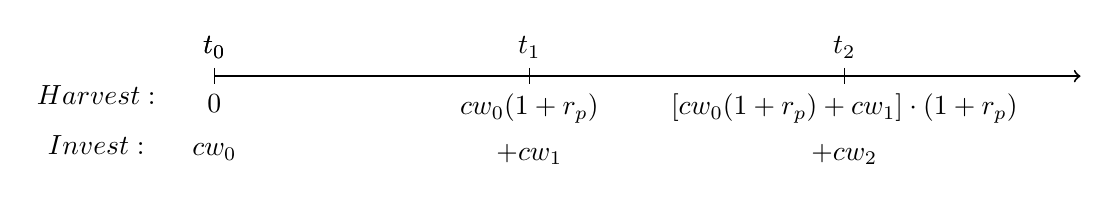
\begin{tikzpicture}
		\draw [->, line width=0.25mm] (0,0) -- (11,0);
		\foreach \x in {0,4,8}
			\draw (\x cm,3pt) -- (\x cm, -3pt);
		\draw (0,0) node[below=21pt] {$ cw_0 $} node[above=3pt] {$ t_0 $};
    	\draw (4,0) node[below=21pt] {$ +cw_1 $} node[above=3pt] {$ t_1 $};
    	\draw (8,0) node[below=21pt] {$ +cw_2 $} node[above=3pt] {$ t_2 $};
		\draw (0,0) node[below=3pt] {$ 0 $} node[above=3pt] {$ t_0 $};
    	\draw (4,0) node[below=3pt] {$ cw_0(1+r_p) $};
    	\draw (8,0) node[below=3pt] {$ \left[cw_0(1+r_p) + cw_1 \right] \cdot (1+r_p) $};
	    \draw (-1.5,0) node[below=18pt] {$ Invest: $};
    	\draw (-1.5,0) node[below=0pt] {$ Harvest: $};
	\end{tikzpicture}
	\caption{Law of motion of financial capital. Every period, a certain percentage $c$ of the wage $w_t$ is invested in a retirement portfolio, while the previously invested amount accrues interest at portfolio rate of return $r_p$.}
	\label{fig:invdiag}
\end{figure}


\subsection{Investment strategies}

Below, we present the life-cycle investment strategies to be benchmarked.

\subsubsection{Homogeneous life-cycles}

Homogeneous life-cycles are strategies, common to all individuals, regardless of their idiosyncratic characteristics. We benchmark strategies given by equations \ref{eq:markowitz}, \ref{eq:stominus}, \ref{eq:cgm}, and an aggressive portfolio allocation, offered by Turkish banks ($60\%$ in stocks, $40\%$ in bonds). Figure \ref{fig:defaults} illustrates the stock shares in these investment strategies.


\begin{figure}[h!]
	\centering
	\includegraphics[scale=0.4]{figs/defaults.pdf}
	\caption{Share of stocks in a portfolio at every age, proposed by homogeneous life-cycle strategies}
	\label{fig:defaults}
\end{figure}


\subsubsection{Heterogeneous life-cycles}

Heterogeneous life-cycles take idiosyncratic characteristics into consideration. We benchmark strategies by \citet{bodie} (see Equation \ref{eq:bodie}), and \citet{munk} (see Equation \ref{eq:munkno}), which are illustrated in Figure \ref{fig:individs} by blue and red curves respectively. The dashed lines illustrate the $68\%$-confidence interval ($\pm 1\sigma$). The figure proposes younger investors to allocate all of their funds in stocks, and gradually, through life, decrease their share in the portfolio --- the more risk-averse they are or the flatter their wage curve is, the sooner. It also shows that, other things being equal, \citet{munk}'s strategy without housing, is less aggressive than \citet{bodie}'s, which is consistent with equations \ref{eq:bodie} and \ref{eq:munkno}. 

\begin{figure}[h!]
	\centering
    \begin{subfigure}{0.45\textwidth}
		\centering
		\includegraphics[scale=0.3]{figs/individuals15.pdf}
		\caption{$\gamma = 1.5$}
	\end{subfigure}
	\hfill
    \begin{subfigure}{0.45\textwidth}
		\centering
		\includegraphics[scale=0.3]{figs/individuals3.pdf}
		\caption{$\gamma = 3$}
	\end{subfigure}
\end{figure}
\begin{figure}[H]\ContinuedFloat
    \begin{subfigure}{0.45\textwidth}
		\centering
		\includegraphics[scale=0.3]{figs/individuals5.pdf}
		\caption{$\gamma = 5$}
	\end{subfigure}
	\hfill
    \begin{subfigure}{0.45\textwidth}
		\centering
		\includegraphics[scale=0.3]{figs/individuals10.pdf}
		\caption{$\gamma = 10$}
	\end{subfigure}
	\caption{Shares of stocks in a portfolio, suggested by \citet{bodie} (blue curves) and \citet{munk} (red curves) in the absence of housing investment, for heterogeneous agents. The optimal allocations at every age depend on the previous realizations of volatile stock returns --- the dashed lines illustrate the confidence intervals for $\pm \sigma$. Higher risk-aversion, steeper wage curve and smaller stock-income correlation lead to less aggressive investment in stocks, and vice versa. }
	\label{fig:individs}
\end{figure}


Figure \ref{fig:munkh} shows the stock and house shares, suggested by \citet{munk} for flat, moderate and steep labor income curves, low, moderate and high stock-wage correlations, and different levels of risk aversion. It confirms that steeper labor income curves results in a larger share of stocks in portfolio, and the more risk averse individuals are, the sooner they decrease both housing and stock investment, and buy more bonds.

\begin{figure}[H]
	\centering
    \begin{subfigure}{0.45\textwidth}
		\centering
		\includegraphics[scale=0.3]{figs/smunkhouse15.pdf}
		\caption{Stocks for $\gamma = 1.5$}
	\end{subfigure}
	\hfill
    \begin{subfigure}{0.45\textwidth}
		\centering
		\includegraphics[scale=0.3]{figs/hmunkhouse15.pdf}
		\caption{Housing for $\gamma = 1.5$}
	\end{subfigure}
\end{figure}
\begin{figure}[H]\ContinuedFloat
    \begin{subfigure}{0.45\textwidth}
		\centering
		\includegraphics[scale=0.3]{figs/smunkhouse3.pdf}
		\caption{Stocks for $\gamma = 3$}
	\end{subfigure}
	\hfill
    \begin{subfigure}{0.45\textwidth}
		\centering
		\includegraphics[scale=0.3]{figs/hmunkhouse3.pdf}
		\caption{Housing for $\gamma = 3$}
	\end{subfigure}
\end{figure}
\begin{figure}[H]\ContinuedFloat
    \begin{subfigure}{0.45\textwidth}
		\centering
		\includegraphics[scale=0.3]{figs/smunkhouse5.pdf}
		\caption{Stocks for $\gamma = 5$}
	\end{subfigure}
	\hfill
    \begin{subfigure}{0.45\textwidth}
		\centering
		\includegraphics[scale=0.3]{figs/hmunkhouse5.pdf}
		\caption{Housing for $\gamma = 5$}
	\end{subfigure}
\end{figure}
\begin{figure}[H]\ContinuedFloat
    \begin{subfigure}{0.45\textwidth}
		\centering
		\includegraphics[scale=0.3]{figs/smunkhouse10.pdf}
		\caption{Stocks for $\gamma = 10$}
	\end{subfigure}
	\hfill
    \begin{subfigure}{0.45\textwidth}
		\centering
		\includegraphics[scale=0.3]{figs/hmunkhouse10.pdf}
		\caption{Housing for $\gamma = 10$}
	\end{subfigure}
	\caption{Munk's stock and housing shares for different wage growth, stock-wage correlation and risk aversion levels}
	\label{fig:munkh}
\end{figure}

Tables with portfolio allocations can be reproduced using the data and methodology explained in this paper in detail.

% WELFARE COMPARISON
%%%%%%%%%%%%%%%%%%%%%%%%%%%%%%%%%%%%%%%%%%%%%%%%%%%%%%%%%%%%%%%%%%%%%%%%%%%%%%%%%%%%%%%%%%%%%%%%%%%%%%%%%%%%%%%%%%%%%%%%%%%%%%%%%%%%%
\section{Welfare comparison and results}
\label{welfare}

In this section, we calculate the accumulated wealth for every investment option above and benchmark the resulting expected utilities.

\subsection{Accumulated wealth}

After the lifetime of investing, households accumulate different levels of wealth. Tables \ref{table:wealthhom} and \ref{table:wealthhet} summarize the mean and standard deviation of 10,000 stock and house price realizations from a Monte Carlo simulation. It is important to note that the values are $\chi^2$-distributed since they depend on two random normal variables --- stock and house prices.

\begin{table}[h!]
	\centering
	\caption{Monte Carlo Results of Accumulated Wealth for Homogeneous Investment Strategies}
	\label{table:wealthhom}
	\begin{tabular}[c]{|l|c|c|c|}
		\hline
		 wages& steep & moderate & flat\\
		\hline
Markowitz			&  343  &   201&   130\\
							& (87)  &  (50)&   (35)\\
$100-age$					&  449  &   261&  175\\  
							& (442) & (246)& (191)\\
Cocco et al.				&  556  &   320&  222\\  
							&(1,348)& (728)& (611)\\
Turkish banks			 	&  483  &   280&  189\\  
							&  (619)& (348)& (264)\\
	\hline
	\end{tabular}
\end{table}

\begin{table}[h!]
	\centering
	\caption{Monte Carlo Results of Accumulated Wealth for Heterogeneous Investment Strategies}
	\label{table:wealthhet}
	\begin{tabular}[c]{|l|ccc|ccc|ccc|}
		\hline
		 wages& \multicolumn{3}{c|}{steep} & \multicolumn{3}{c|}{moderate} & \multicolumn{3}{c|}{flat}\\
		\hline
		$\rho_{ws}$&high&moderate&low&high&moderate&low&high&moderate&low\\
		\hline
	\multicolumn{10}{|c|}{$\gamma=1.5$}\\
		\hline
Bodie et al.			 	&-&  544  &-&-&   315&-&-&  206&-\\  
							&-&  (756)&-&-& (433)&-&-& (281)&-\\
Munk (no housing)			&  524  &  531&   538&  304&  309&  312&  199&  202&  204\\
							&  (663)&  (700)&  (733)&  (379)&  (400)&  (418)&  (249)&  (263)&  (275)\\
Munk (housing)				&  403  &  416&  430&  235&  243&  251&  154&  159&  165\\
							&  (495)&  (541)&  (591)&  (280)&  (306)&  (334)&  (201)&  (219)&  (239)\\
	\hline
	\multicolumn{10}{|c|}{$\gamma=3$}\\
	\hline
Bodie et al.			 	&-&  484  &-&-&281  &-&-& 182&-\\
							&-&  (479)&-&-&(276)&-&-& (176)&-\\
Munk (no housing)			&  449&  468&  482&  262&  272&  280&  168&  176&  181\\
							&  (352)&  (419)&  (473)&  (204)&  (241)&  (272)&  (129)&  (154)&  (174)\\
Munk (housing)				&  514&  534&  546&  299&  310&  317&  194&  202&  206\\
							&  (711)&  (778)&  (826)&  (407)&  (446)&  (473)&  (264)&  (289)&  (307)\\
	\hline
	\multicolumn{10}{|c|}{$\gamma=5$}\\

		\hline
Bodie et al.			 	&-& 450&-&-& 262&-&-& 168&-\\
							&-& (344)&-&-& (199)&-&-& (125)&-\\
Munk (no housing)			&  377&  423&  448&  221&  247&  262&  140&  158&  168\\
							&  (149)&  (263)&  (343)&  (87)&  (153)&  (198)&  (54)&  (95)&  (125)\\
Munk (housing)				&  497&  509&  520&  289&  296&  302&  187&  192&  196\\
							&  (513)&  (563)&  (608)&  (295)&  (324)&  (349)&  (189)&  (208)&  (224)\\
	\hline
	\multicolumn{10}{|c|}{$\gamma=10$}\\

		\hline
Bodie et al.			 	&-&  402&-&-&  235&-&-& 149&- \\
							&-&  (212)&-&-&  (124)&-&-&  (76)&- \\
Munk (no housing)			&  302&  345&  401&  178&  203&  235&  113&  128&  149\\
							&    (1)&   (80)&  (212)&    (1)&   (47)&  (124)&    (1)&   (28)&   (76)\\
Munk (housing)				&  418&  446&  465&  244&  260&  271&  156&  167&  174\\
							&  (252)&  (339)&  (405)&  (147)&  (196)&  (234)&   (91)&  (123)&  (148)\\
	\hline
	\end{tabular}
\end{table}


\subsection{Annuities}

Retired individuals will sell all of their accumulated wealth to buy annuities and consume them fully until their death, enjoying the utility of this consumption. Recall that we ignore bequest motives and savings after the retirement. We define annuities by dividing the total wealth before retirement by the discount factor $1 + \sum^{100}_{t=66}\frac{p_t}{(1+r_f)^{t-65}}$. Using survival probabilities, obtained from TUIK, and risk-free rate of return, described in the previous chapter, we calculate the discount factor as $13.73$. The annuities are obtained by dividing all the values in the Tables \ref{table:wealthhom} and \ref{table:wealthhet} by $13.73$. 


\subsection{Expected utilities}
Recall that we have defined the wages in real terms, dividing the nominal wages by CPI. Therefore we can plug the values, obtained above, to the CRRA utility function as consumption level. Table \ref{table:util} provides mean and standard deviation of accumulated wealth from different scenarios of a Monte Carlo experiment, mentioned above. Note that the distributions are heavily skewed to the left.

\newgeometry{left=1.5cm}
\begin{table}[h!]
	\centering
	\caption{A: Summary of Expected Utilities from Simulation for $\gamma=1.5$}
	\label{table:util}
	\begin{tabular}[c]{|l|ccc|ccc|ccc|}
		\hline
		 wages& \multicolumn{3}{c|}{steep} & \multicolumn{3}{c|}{moderate} & \multicolumn{3}{c|}{flat}\\
		\hline
		$\rho_{ws}$&high&moderate&low&high&moderate&low&high&moderate&low\\
		\hline
Markowitz					&-2.515&-2.515&-2.515&-3.282&-3.282&-3.282&-4.096&-4.096&-4.096\\
							&(0.314)&(0.314)&(0.314)&(0.403)&(0.403)&(0.403)&(0.547)&(0.547)&(0.547)\\
$100-age$					&-2.593&-2.593&-2.593&-3.374&-3.374&-3.374&-4.285&-4.285&-4.285\\
							&(0.874)&(0.874)&(0.874)&(1.116)&(1.116)&(1.116)&(1.568)&(1.568)&(1.568)\\
Cocco et al.				&-2.889&-2.889&-2.889&-3.734&-3.734&-3.734&-4.899&-4.899&-4.899\\
							&(1.299)&(1.299)&(1.299)&(1.623)&(1.623)&(1.623)&(2.333)&(2.333)&(2.333)\\
Turkish banks			 	&-2.772&-2.772&-2.772&-3.608&-3.608&-3.608&-4.612&-4.612&-4.612\\
							&(1.187)&(1.187)&(1.187)&(1.531)&(1.531)&(1.531)&(2.122)&(2.122)&(2.122)\\
Bodie et al.			 	&-3.389&-3.389&-3.389&-4.389&-4.389&-4.389&-5.695&-5.695&-5.695\\
							&(2.352)&(2.352)&(2.352)&(3.048)&(3.048)&(3.048)&(4.252)&(4.252)&(4.252)\\
Munk (no housing)			&-3.355&-3.415&-3.476&-4.346&-4.435&-4.499&-5.61&-5.729&-5.841\\
							&(2.334)&(2.403)&(2.506)&(3.096)&(3.242)&(3.304)&(4.253)&(4.37)&(4.553)\\
Munk (housing)				&-3.043&-3.071&-3.103&-3.952&-3.987&-4.027&-5.105&-5.159&-5.22\\
							&(1.327)&(1.398)&(1.472)&(1.71)&(1.802)&(1.899)&(2.387)&(2.519)&(2.656)\\
	\hline
	\end{tabular}
\end{table}
\begin{table}[h!]\ContinuedFloat
	\centering
	\caption{B: Summary of Expected Utilities from Simulation for $\gamma=3$}
	\label{table:util}
	\begin{tabular}[c]{|l|ccc|ccc|ccc|}
		\hline
		 wages& \multicolumn{3}{c|}{steep} & \multicolumn{3}{c|}{moderate} & \multicolumn{3}{c|}{flat}\\
		\hline
		$\rho_{ws}$&high&moderate&low&high&moderate&low&high&moderate&low\\
		\hline
Markowitz					&-0.006&-0.006&-0.006&-0.017&-0.017&-0.017&-0.042&-0.042&-0.042\\
							&(0.003)&(0.003)&(0.003)&(0.009)&(0.009)&(0.009)&(0.023)&(0.023)&(0.023)\\
$100-age$					&-0.011&-0.011&-0.011&-0.031&-0.031&-0.031&-0.09&-0.09&-0.09\\
							&(0.016)&(0.016)&(0.016)&(0.045)&(0.045)&(0.045)&(0.151)&(0.151)&(0.151)\\
Cocco et al.				&-0.023&-0.023&-0.023&-0.062&-0.062&-0.062&-0.216&-0.216&-0.216\\
							&(0.042)&(0.042)&(0.042)&(0.115)&(0.115)&(0.115)&(0.469)&(0.469)&(0.469)\\
Turkish banks			 	&-0.019&-0.019&-0.019&-0.055&-0.055&-0.055&-0.17&-0.17&-0.17\\
							&(0.043)&(0.043)&(0.043)&(0.124)&(0.124)&(0.124)&(0.418)&(0.418)&(0.418)\\
Bodie et al.			 	&-0.372&-0.372&-0.372&-0.579&-0.579&-0.579&-1.182&-1.182&-1.182\\
							&(22.2)&(22.2)&(22.2)&(25.6)&(25.6)&(25.6)&(53.1)&(53.1)&(53.1)\\
Munk (no housing)			&-0.04&-0.063&-0.212&-0.099&-0.192&-0.427&-0.287&-0.963&-3.585\\
							&(0.507)&(0.608)&(10.291)&(0.665)&(3.287)&(15.333)&(1.914)&(28.294)&(176.463)\\
Munk (housing)				&-0.515&-0.289&-1.132&-3.637&-3.403&-1.226&-55.076&-7.09&-507.406\\
							&(39.222)&(11.653)&(86.736)&(312.4)&(291)&(50.427)&(3832)&(533.61)&(50503)\\
	\hline
	\end{tabular}
\end{table}
\begin{table}[h!]\ContinuedFloat
	\centering
	\caption{C: Summary of Expected Utilities from Simulation for $\gamma=5$}
	\label{table:util}
	\begin{tabular}[c]{|l|ccc|ccc|ccc|}
		\hline
		 wages& \multicolumn{3}{c|}{steep} & \multicolumn{3}{c|}{moderate} & \multicolumn{3}{c|}{flat}\\
		\hline
		$\rho_{ws}$&high&moderate&low&high&moderate&low&high&moderate&low\\
		\hline
Markowitz					&0&0&0&0&0&0&0&0&0\\
							&(0)&(0)&(0)&(0)&(0)&(0)&(0.001)&(0.001)&(0.001)\\
$100-age$					&0&0&0&-0.001&-0.001&-0.001&-0.005&-0.005&-0.005\\
							&(0)&(0)&(0)&(0.003)&(0.003)&(0.003)&(0.044)&(0.044)&(0.044)\\
Cocco et al.				&-0.002&-0.002&-0.002&-0.003&-0.003&-0.003&-1.372&-1.372&-1.372\\
							&(0.201)&(0.201)&(0.201)&(0.027)&(0.027)&(0.027)&(90.495)&(90.495)&(90)\\
Turkish banks			 	&0&0&0&-0.003&-0.003&-0.003&-0.039&-0.039&-0.039\\
							&(0.005)&(0.005)&(0.005)&(0.04)&(0.04)&(0.04)&(0.598)&(0.598)&(0.598)\\
Bodie et al.			 	&-0.14&-0.14&-0.14&-1.684&-1.684&-1.684&-34.122&-34.122&-34.122\\
							&(10.141)&(10.141)&(10.141)&(139.3)&(139.3)&(139.3)&(2926)&(2926)&(2926)\\
Munk (no housing)			&-0.007&-0.228&-33879.48&-0.047&-4.169&-3.2&-0.518&-321.58&-11420.369\\
							&(0.226)&(14.403)&(3387924)&(1.387)&(388.399)&(190)&(12.701)&(31692)&(1102401)\\
Munk (housing)				&-0.608&-198.462&-3.52&-6.667&-930.941&-78.93&-23.559&-41341.4&-93.43\\
							&(51.7)&(19257)&(267.51)&(598)&(86349)&(6966)&(1401)&(3920139)&(5322)\\
	\hline
	\end{tabular}
\end{table}
\begin{table}[h!]\ContinuedFloat
	\centering
	\caption{D: Summary of Expected Utilities from Simulation for $\gamma=10$}
	\label{table:util}
	\begin{tabular}[c]{|l|ccc|ccc|ccc|}
		\hline
		 wages& \multicolumn{3}{c|}{steep} & \multicolumn{3}{c|}{moderate} & \multicolumn{3}{c|}{flat}\\
		\hline
		$\rho_{ws}$&high&moderate&low&high&moderate&low&high&moderate&low\\
		\hline
Markowitz					&0&0&0&0&0&0&0&0&0\\
							&(0)&(0)&(0)&(0)&(0)&(0)&(0)&(0)&(0)\\
$100-age$					&0&0&0&0&0&0&0&0&0\\
							&(0)&(0)&(0)&(0)&(0)&(0)&(0.016)&(0.016)&(0.016)\\
Cocco et al.				&0.001&0.001&0.001&-1.32&-1.32&-1.32&843&843&843\\
							&(0.12)&(0.12)&(0.12)&(138.203)&(138.203)&(138.203)&(923)&(923)&(923)\\
Turkish banks			 	&0&0&0&0&0&0&-0.031&-0.031&-0.031\\
							&(0)&(0)&(0)&(0.003)&(0.003)&(0.003)&(1.06)&(1.06)&(1.06)\\
Bodie et al.			 	&0&0&0&-0.002&-0.002&-0.002&-1.432&-1.432&-1.432\\
							&(0.001)&(0.001)&(0.001)&(0.09)&(0.09)&(0.09)&(85.945)&(85.945)&(85.945)\\
Munk (no housing)			&0&0&0&0&0&-0.001&0&0&-0.781\\
							&(0)&(0)&(0.001)&(0)&(0)&(0.086)&(0)&(0)&(56.102)\\
Munk (housing)				&0&-0.001&-19368&-0.002&-0.1&-9661.276&-1.283&-57.043&-3694.293\\
							&(0.001)&(0.051)&(1936894)&(0.106)&(5.981)&(699694)&(75)&(4115)&(281712)\\
	\hline
	\end{tabular}
\end{table}
\restoregeometry

\subsection{Pairwise comparisons}
In this section we provide the pairwise comparisons of utilities for different investment options. Table \ref{table:compareutils} shows percentages of scenarios at which the utilities from some investment options are greater than from the other. We ignored small percentage differences (up to $3\%$) as noise, and interpreted percentages close to $50\%$ as ``no conclusion''.

We can see that homogeneous investment options return same ordering regardless of risk aversion, even though $\gamma$ enters the utility equation. Similarly, steepness of labor income curve does not affect within-group ordering. At the same time, level of risk-aversion, and correlation of wages to stocks, do affect the ordering.


\newgeometry{left=1cm}
\begin{table}[h!]
	\centering
	\caption{A: Utility Comparison for $\gamma=1.5$}
	\label{table:compareutils}
	\begin{tabular}[c]{|l|ccccccc|}
		\hline
		L $\geq$ R			&Markowitz&$100-age$&Cocco et al.&TR Banks&Bodie et al.&Munk (no h.)&Munk (h.)\\
		\hline
Markowitz					&100\%&51\%&60\%&54\%&55\%&55\%&64\%\\
$100-age$					&&100\%&72\%&61\%&58\%&57\%&80\%\\
Cocco et al.				&&&100\%&32\%&55\%&56\%&70\%\\
Turkish banks			 	&&&&100\%&65\%&65\%&95\%\\
Bodie et al.			 	&&&&&100\%&58\% (81\% if $\rho_{ws}=0$)&48\%\\
Munk (no housing)			&&&&&&100\%&46\%\\
Munk (housing)				&&&&&&&100\%\\
	\hline
	\end{tabular}
\end{table}
\begin{table}[h!]\ContinuedFloat
	\centering
	\caption{B: Utility Comparison for $\gamma=3$}
	\label{table:compareutils}
	\begin{tabular}[c]{|l|ccccccc|}
		\hline
		L $\geq$ R			&Markowitz&$100-age$&Cocco et al.&TR Banks&Bodie et al.&Munk (no h.)&Munk (h.)\\
		\hline
Markowitz					&100\%&51\%&60\%&54\%&49\%&48\%&57\%\\
$100-age$					&&100\%&72\%&60\%&56\%&56\%&61\%\\
Cocco et al.				&&&100\%&31\%&51\%&50\%&58\%\\
Turkish banks			 	&&&&100\%&58\%&54\%;57\%;60\% ($\rho_{ws} \searrow$ )&66\%\\
Bodie et al.			 	&&&&&100\%&55\% (70\% if $\rho_{ws}=0$)&55\%\\
Munk (no housing)			&&&&&&100\%&55\%\\
Munk (housing)				&&&&&&&100\%\\
	\hline
	\end{tabular}
\end{table}
\begin{table}[h!]\ContinuedFloat
	\centering
	\caption{C: Utility Comparison for $\gamma=5$}
	\label{table:compareutils}
	\begin{tabular}[c]{|l|ccccccc|}
		\hline
		L $\geq$ R			&Markowitz&$100-age$&Cocco et al.&TR Banks&Bodie et al.&Munk (no h.)&Munk (h.)\\
		\hline
Markowitz					&100\%&51\%&61\%&54\%&50\%&50\%&57\%\\
$100-age$					&&100\%&72\%&61\%&56\%&56\%&62\%\\
Cocco et al.				&&&100\%&30\%&50\%&50\%&59\%\\
Turkish banks			 	&&&&100\%&58\%&53\%;57\%;60\% ($\rho_{ws}\searrow$)&67\%\\
Bodie et al.			 	&&&&&100\%&55\% (70\% if $\rho_{ws}=0$)&54\%\\
Munk (no housing)			&&&&&&100\%&55\%\\
Munk (housing)				&&&&&&&100\%\\
	\hline
	\end{tabular}
\end{table}
\begin{table}[h!]\ContinuedFloat
	\centering
	\caption{D: Utility Comparison for $\gamma=10$}
	\label{table:compareutils}
	\begin{tabular}[c]{|l|ccccccc|}
		\hline
		L $\geq$ R			&Markowitz&$100-age$&Cocco&TR Banks&Bodie&Munk (no h.)&Munk (h.)\\
		\hline
Markowitz					&100\%&51\%&61\%&55\%&43\%&65\%;48\%;42\% ($\rho_{ws}\searrow$)&43\%;46\%;49\% ($\rho_{ws}\searrow$)\\
$100-age$					&&100\%&73\%&61\%&52\%&50\%&53\%($\rho_{ws}=0.4$);57\%\\
Cocco et al.				&&&100\%&30\%&40\%&45\% ($\rho_{ws}=0.4$);40\%&41\%;46\%;51\% ($\rho_{ws}\searrow$)\\
Turkish banks			 	&&&&100\%&47\%&50\% ($\rho_{ws}=0.4$);47\%&48\%;54\%;58\% ($\rho_{ws}\searrow$)\\
Bodie et al.			 	&&&&&100\%&62\%;99\% ($\rho_{ws}=0$)&42\%;45\%;47\% ($\rho_{ws}\searrow$)\\
Munk (no housing)			&&&&&&100\%&38\%;45\%;47\% ($\rho_{ws} \searrow$)\\
Munk (housing)				&&&&&&&100\%\\
	\hline
	\end{tabular}
\end{table}


\restoregeometry

The main comparison results are as follows:

\begin{itemize}

\item Naive life-cycle investment portfolio $(100-age)\%$ overperforms all investment options except for Markowitz.
\item Cocco et al.'s $(200-2.5\cdot age)\%$ performs worse than other homogeneous portfolios.
\item All models perform better for higher risk aversion and worse for lower risk aversion.
\item Munk's solution performs worse for flat wages than for steep wages.
\item When $\rho_{ws}=0$, Bodie's solution is equivalent to Munk's solution without housing.
\item Munk's solution with housing performs as well or worse than other options most of the time, except for higly risk-averse individuals, and especially for high wage-stock correlations --- in these cases, investing in housing is the best option. 
\item Munk's solution without housing outperforms other strategies as risk aversion gets higher.
\item Fixed moderate Turkish bank's investment suggestion, outperforms Cocco et al.'s lifecycle heuristic 70\% of the time.
\item For risk-takers ($\gamma < 5$), heterogeneous outcomes are better for steep and moderate labor income curves.
\end{itemize}

% CONCLUSION 
%%%%%%%%%%%%%%%%%%%%%%%%%%%%%%%%%%%%%%%%%%%%%%%%%%%%%%%%%%%%%%%%%%%%%%%%%%%%%%%%%%%%%%%%%%%%%%%%%%%%%%%%%%%%%%%%%%%%%%%%%%%%%%%%%%%%%

\section{Conclusion}
\label{conclusion}

In this paper we have reviewed the concept of "life-cycle investment" and summarized the common models and heuristics. We have presented our model as an application of Munk's (2016) recent findings and Olear's (2016) simulation techniques into Turkish retirement market. We have collected historical data to calibrate and estimate the best parameters to be used in our simulation. Using these parameters, we have constructed heterogeneous agents, who worked and invested throughout their lifetime. We considered different investment models that our hypothetical agents would use and calculated the resulting investment capitals. Finally, we have calculated and compared the welfare effects of all popular models to the individualized Munk's solutions. We have concluded that for rich-to-middle class risk-loving citizens, the individiualized strategies considerably increase their welfare. Moreover, the solutions we proposed can be solved analytically without complex dynamic optimizations, and therefore are easy to interpret to households. We also found that even naive life-cycle investment heuristics perform better than fixed lifetime investments. Our simulation showed that for risk-averse individuals with volatile wages, it is best to invest in housing in a proportion proposed by Munk. We propose these models to Turkish pension providers and to Turkish working-age households belonging to middle-to-upper class, as these options will increase their retirement welfare considerably.

% BIBLIOGRAPHY
%%%%%%%%%%%%%%%%%%%%%%%%%%%%%%%%%%%%%%%%%%%%%%%%%%%%%%%%%%%%%%%%%%%%%%%%%%%%%%%%%%%%%%%%%%%%%%%%%%%%%%%%%%%%%%%%%%%%%%%%%%%%%%%%%%%%%
\section{References}
\begin{thebibliography}{}
\bibitem[Markowitz(1952)]{markowitz} Markowitz H. (1952). Portfolio Selection. \textit{The Journal of Finance}, 7(1), 77-91.
\bibitem[Tobin(1958)]{tobin} Tobin J.(1958). Liquidity Preference as Behavior Towards Risk. \textit{The Review of Economic Studies}, 25(2), 65-86.
\bibitem[Merton(1971)]{merton} Merton R.C. (1971). Optimum Consumption and Portfolio Rules in a Continuous-Time Model. \textit{Journal of Economic Theory}, 3, 373-413.
\bibitem[Samuelson(1969)]{samuelson} Samuelson, Paul A. (1969). Lifetime Portfolio Selection by Dynamic Stochastic Programming. \textit{Review of Economics and Statistics}, 51(3), 239-246.
\bibitem[Canner et al.(1994)]{canner} Canner, N., Mankiw, N.G., Weil, D.N. (1997). An Asset Allocation Puzzle. \textit{The American Economic Review}, 87(1), 181-191.
\bibitem[Bodie et al.(1992)]{bodie}Bodie, Z., Merton, R.C., Samuelson, W.F. (1992). Labor Supply Flexibility and Portfolio Choice in a Life-Cycle Model. \textit{Journal of Economic Dynamics and Control}, 16(3-4), 427-449. 
\bibitem[Cocco et al.(2005)]{cgm} Cocco, J.F., Gomes, F.J., Maenhout P.J. (2005). Consumption and Portfolio Choice over the Life Cycle. \textit{The Review of Financial Studies}, 18(2), 491-533. 
\bibitem[Chang et al.(2014)]{chang} Chang, Y., Hong, J.H., Karabarbounis, M. (2014). Labor-Market Uncertainty and Portfolio Choice Puzzles. \textit{Working Papers, Federal Reserve Bank of Richmond}, 14(13).
\bibitem[Cocco(2004)]{cocco} Cocco, J.F. (2004). Portfolio Choice in the Presence of Housing. \textit{The Review of Financial Studies}, 18(2), 537-567.
\bibitem[Flavin and Yamashita(2002)]{flavin} Flavin M., Yamashita T. (2002). Owner-Occupied Housing and the Composition of the Household Portfolio. \textit{The American Economic Review}, 1, 345-362.
\bibitem[Munk(2016)]{munk} Munk C. (2016). A Mean-Variance Benchmark for Household Portfolios over the Life Cycle. \textit{Working Papers, Copenhagen Business School, Department of Finance}.
\bibitem[Ascheberg et al.(2013)]{ascheberg} Ascheberg, M., Kraft, H., Munk, C., Weiss, F. (2013). The Joint Dynamics of Labor Income, Stock Prices, and House Prices and the Implications for Household Decisions. \textit{Working Papers, Dauphine Universite Paris, International Workshop on Pension, Insurance and Saving}.
\bibitem[Campbell et al.(1999)]{ccgm} Campbell, J., Cocco, J.F., Gomes, F.J., Maenhout, P.J. (1999). Investing Retirement Wealth: A Life-Cycle Model. \textit{Working Papers, National Bureau of Economic Research}, 439-482.
\bibitem[Olear(2016)]{olear} Olear G.M. (2016). Benefits of Individualized Lifecycle Investing: The Impact of Individual Wage Profile \& Housing Wealth. \textit{Master's Thesis, Tilburg University, School of Economics and Management}.
\bibitem[Turkish Statistical Institute's Household Budget Survey(2003-2014)]{tuik} TUIK (2003-2014). Hanehalki Butce Anketi. \textit{Turkish Statistical Institute}.
\bibitem[Aktug et al.(2017)]{aktug} Aktuğ, E., Kuzubaş, T.U., Torul, O. (2017). An Investigation of Labor Income Profiles in Turkey. \textit{Working Papers, Boğaziçi  University, Department of Economics}.
\bibitem[Ben-Porath(1967)]{benporath} Ben-Porath, Y. (1967). The  Production  of  Human  Capital  and  the  Life-Cycle  of  Earnings. \textit{Journal of Political Economy}, 75, 352-365.
\bibitem[Torul and Oztunali(2018)]{torul} Torul, O., Öztunalı, O. (2018). On Income and Wealth Inequality in Turkey. \textit{Working Papers, Boğaziçi University, Department of Economics}.
\bibitem[OECD(2018)]{oecd} OECD(2018). Long-term interest rates forecast (indicator). \textit{https://data.oecd.org}
\bibitem[Turkish Statistical Institute's Data Bank(2018)]{tuik2} TUIK (2018). General Statistics. \textit{http://www.turkstat.gov.tr}.
\bibitem[Turkish Central Bank's Inflation Report (2018)]{tcmb} TCMB (2018). Enflasyon Raporu. \textit{http://www.tcmb.gov.tr}.
\end{thebibliography}

% APPENDIX A
%%%%%%%%%%%%%%%%%%%%%%%%%%%%%%%%%%%%%%%%%%%%%%%%%%%%%%%%%%%%%%%%%%%%%%%%%%%%%%%%%%%%%%%%%%%%%%%%%%%%%%%%%%%%%%%%%%%%%%%%%%%%%%%%%%%%%
\newpage
\begin{appendix}

\section{Ascheberg's correlation structure}
\label{ascheberg}

The structure that returns desired correlation coefficients $\rho_{SL}$, $\rho_{SH}$ and $\rho_{HL}$ is as follows:

\begin{subequations}
	\begin{equation}
		\frac{\Delta S_{t+1}}{S_t} = \mu_S + \sigma_S \cdot \epsilon_{St}
	\end{equation}
	\begin{equation}
		\frac{\Delta H_{t+1}}{H_t} = \mu_H + \sigma_H \cdot \left(\rho_{SH}\epsilon_{St} + (\sqrt{1-\rho^2_{SL}})\epsilon_{Ht}\right)
	\end{equation}
	\begin{equation}
		\frac{\Delta Y_{t+1}}{Y_t} = \mu_L + \sigma_L \cdot \left(\rho_{SL}\epsilon_{St} + \left(\frac{\rho_{HL} - \rho_{SH}\rho_{SL}}{\sqrt{1-\rho^2_{SH}}}\right)\epsilon_{Ht} + \left(\sqrt{1-\rho^2_{SL}-(\frac{\rho_{HL} - \rho_{SH}\rho_{SL}}{\sqrt{1-\rho^2_{SH}}})^2}\right)\epsilon_{Lt}\right)
	\end{equation}
\end{subequations}

To derive this, let $\Sigma$ be a correlation matrix of a vector $X = (x_1, x_2, ..., x_K)$. Also, let $\Sigma = LL'$ be a Cholesky decomposition of this matrix.

Notice that the variance-covariance matrix of an i.i.d. random vector $\Omega = (\epsilon_1, \epsilon_2, ..., \epsilon_K)$ with variances equal to $1$, is an identity matrix. Thus, the product $L\Omega$ has the same correlation structure as $X$:

\begin{center}
  $cov(L\Omega) = E[(L\Omega)(L\Omega)'] = E[L\Omega\Omega'L']$,\\
  $cov(L\Omega) = L \cdot E[\Omega\Omega'] \cdot L' = L \cdot var(\Omega) \cdot L'$,\\
  $cov(L\Omega) = L\cdot I \cdot L' = LL' = \Sigma$
\end{center}

The conclusion comes from the fact that the Cholesky decomposition of a correlation matrix $R$:

\begin{center}
	$R = \begin{bmatrix}
					1 & \rho_{SH} & \rho_{SL} \\
					\rho_{SH} & 1 & \rho_{HL} \\
					\rho_{SL} & \rho_{HL} & 1
			\end{bmatrix}
	$
\end{center}

can be easily calculated to be equal to $Q$:

\begin{center}
	$Q = \begin{bmatrix}
					1 & 0 & 0 \\
					\rho_{SH} & \sqrt{1-\rho^2_{SH}} & 0 \\
					\rho_{SL} & \frac{\rho_{HL} - \rho_{SH}\rho_{SL}}{\sqrt{1-\rho^2_{SH}}} & \sqrt{1-\rho^2_{SL}-(\frac{\rho_{HL} - \rho_{SH}\rho_{SL}}{\sqrt{1-\rho^2_{SH}}})^2}
			\end{bmatrix}
	$
\end{center}


% APPENDIX B
%%%%%%%%%%%%%%%%%%%%%%%%%%%%%%%%%%%%%%%%%%%%%%%%%%%%%%%%%%%%%%%%%%%%%%%%%%%%%%%%%%%%%%%%%%%%%%%%%%%%%%%%%%%%%%%%%%%%%%%%%%%%%%%%%%%%%
\newpage
\section{Parameter Calibrations}
\label{paramcalib}

\subsection{Stock returns}
\label{paramcalibx}
We use log differences on our monthly stock price data to obtain historical monthly rates of return. The Augmented Dickey-Fuller test strongly shows that the modified series is stationary at $1\%$ significance level.

\begin{figure}[h!]
	\centering
	\includegraphics[scale=0.3]{figs/bistdiff.pdf}
	\caption{Historical monthly rates of return on stocks}
	\label{fig:bistdiff}
\end{figure}

We use Akaike Information Criterion to find the optimal lag order for ARIMA estimation --- $p=q=2$.

Performing ARIMA(2,0,2) estimation, we obtain the long-term forecasted monthly rate of return $\mu^S_{mon} = 0.541\%$ and volatility $\sigma^S_{mon} = 11.1\%$.

Finally, we annualize these values as follows:

\begin{equation}
	\mu_S = (1 + \mu^S_{mon})^{12} - 1= 6.69\%
\end{equation}

\begin{equation}
	\sigma_S = \sigma^S_{mon} \cdot \sqrt{12} = 38.44\%
\end{equation}

\subsection{Housing returns}
\label{paramcaliby}
Similarly, we log-differentiate monthly house prices to obtain growth rates. The house market collapse of 2008 brings large external shock, causing the Augmented Dickey-Fuller test to only find stationarity at $10\%$ significance level for 3 lags at most.

\begin{figure}[h!]
	\centering
	\includegraphics[scale=0.3]{figs/reidindiff.pdf}
	\caption{Historical monthly rates of return on housing}
	\label{fig:reidindiff}
\end{figure}

Again, using Akaike Information Criterion, we find $p=q=1$.

ARIMA(1,0,1) estimation provides long-term forecasts for monthly rate of return and volatility as $\mu^H_{mon} = 0.06\%$ and $\sigma^H_{mon} = 1.57\%$.

Annualization gives:

\begin{equation}
	\mu_H = (1 + \mu^H_{mon})^{12} - 1= 0.67\%
\end{equation}

\begin{equation}
	\sigma_H = \sigma^H_{mon} \cdot \sqrt{12} = 5.42 \%
\end{equation}


\subsection{Labor income volatility}
\label{paramcalibz}
The Augmented Dickey-Fuller test returns stationarity for up to 9 lags at $5\%$ significance level. 

\begin{figure}[h!]
	\centering
	\includegraphics[scale=0.3]{figs/wagediff.pdf}
	\caption{Historical monthly wage growth rates}
	\label{fig:wagediff}
\end{figure}

Akaike Information Criterion suggests $p=5$ and $q=2$.

ARIMA(5,0,2) estimation gives monthly volatility $\sigma^L_{mon} = 1.04\%$, which annualizes as follows:

\begin{equation}
	\sigma_L = \sigma^L_{mon} \cdot \sqrt{12} = 3.59 \%
\end{equation}


\subsection{Wage regression results}
\label{paramcalibt}

The regressions of wage growth rates by age with kinks at 40 and 55, return the following coefficients.

\begin{table}[H]
	\centering
	\caption[]{Wage regression results by age}
	\begin{tabular}[c]{lccc}
		\hline
		&flat&moderate&steep\\
		\hline
		(intercept)&0.1\%&0.4\%&1.5\%\\
		d40&-0.7\%&3.3\%&0.7\%\\
		d55&1.4\%&0.9\%&-0.4\%\\
		\hline
	\end{tabular}
\end{table}

The growth rates can be calculated using these coefficients. Note that we have rounded the growth rates for the flat wages to $0$. Figure \ref{fig:heterwage} illustrates how the estimated rates fit the data:

\begin{figure}[h!]
	\centering
	\includegraphics[scale=0.3]{figs/heterwage.pdf}
	\caption{Fitted values from wage regressions}
	\label{fig:heterwage}
\end{figure}


% APPENDIX C
%%%%%%%%%%%%%%%%%%%%%%%%%%%%%%%%%%%%%%%%%%%%%%%%%%%%%%%%%%%%%%%%%%%%%%%%%%%%%%%%%%%%%%%%%%%%%%%%%%%%%%%%%%%%%%%%%%%%%%%%%%%%%%%%%%%%%
%\newpage
%\section{appendixname}
%\label{appendix label}




\end{appendix}





\end{document}  






%%%%%%%%%%%%%%%%%%%%%%%%%%%%%%%%%%%%%%%%%%%%%%%%%%%%%%%%%%%%%%%%%%%%%%%%%%%%%%%%%%%%%%%%%%%%%%%%%%%%%%%%%%%%%%%%








